\documentclass{article}

\usepackage[letterpaper, portrait, margin=1.5in]{geometry}

\usepackage{fancyhdr}
\usepackage{ragged2e}
\usepackage{graphicx}
\usepackage{caption}
\usepackage{amsmath}
\usepackage{rotating}

\usepackage{listings}
\usepackage{color}

\definecolor{dkgreen}{rgb}{0,0.6,0}
\definecolor{gray}{rgb}{0.5,0.5,0.5}
\definecolor{mauve}{rgb}{0.58,0,0.82}

\lstset{frame=tb,
  language=Java,
  aboveskip=3mm,
  belowskip=3mm,
  showstringspaces=false,
  columns=flexible,
  basicstyle={\small\ttfamily},
  numbers=none,
  numberstyle=\tiny\color{gray},
  keywordstyle=\color{blue},
  commentstyle=\color{dkgreen},
  stringstyle=\color{mauve},
  breaklines=true,
  breakatwhitespace=true,
  tabsize=4
}

\setcounter{secnumdepth}{1}

\usepackage{chngcntr}
\counterwithin{figure}{section}

\renewcommand*{\thepage}{C\arabic{page}}

\pagestyle{fancy}
\lhead{ACME Robotics}
\chead{\#8367}
\rhead{\ifcontents Contents \else Week \thesection \fi}

\newif\ifcontents
\contentstrue

\makeatletter
\renewcommand{\@seccntformat}[1]{}
\makeatother
\begin{document}

\subsection{X-rail mounting work around}
%! Figure out a way to mount the X-rail.
With the new outside plates now cut, the team could begin the final stages of fabricating the robot. There was a problem however, the part that was supposed to be bent over to mount the X-rail from the outside drive plate had broken off during the bending process. This caused the team to learn the hard way that aluminum is not suited for 90 degree bends. To overcome this problem, Jon bolted two Tetrix brackets to the inside of the outside drive plate. This acted almost exactly as the originally mounts would have. Jon did it this way because it was quick, simple, and functional. With a "robot done" deadline fast approaching, this was likely the best solution. While this was neither an elegant or permanent solution, it was at least functional.

\begin{figure}
    \centering
    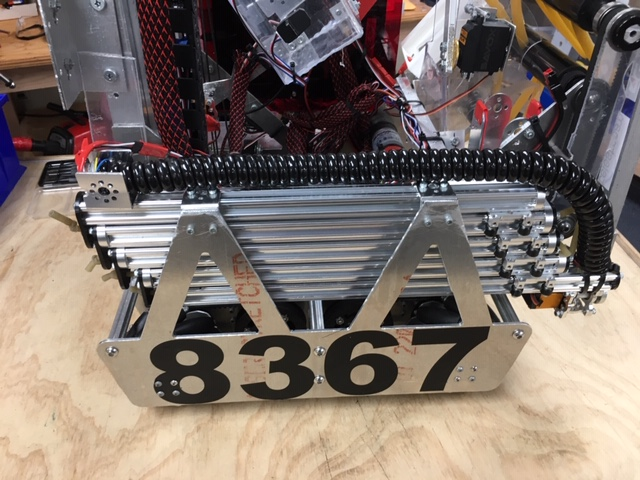
\includegraphics[height=6cm]{18_12-31/images/X-Rail Mount.JPG}
    \caption{X-Rail Bracket Mounts}
    \label{X-Rail Mounts}
\end{figure}



\subsection{Re-Constructing Robot}
%! Re-constructing Robot version 2.0.
After the majority of the newly fabricated parts were completed, we began building version 2.0. The build process the second time around was much faster and went very smooth. We completed the reconstruction with in two meetings, and then began the long and tedious process of wiring everything up. As a team we have learned from past experience that wiring and organization is very important for a functional robot. Organization allows for easy fixes when necessary and creates no confusion when working through software and hardware issues, this is an area that in the past has been neglected. But we have dedicated time and effort to make sure that wiring is cosmetically pleasing and concise. 

\end{document}